%!TEX program = lualatex

\documentclass{UDEbeamerEN}

\usepackage{ifluatex}
\ifluatex
  \usepackage{fontspec}
  \usepackage{polyglossia} % babel replacement for use with fontspec
  \setdefaultlanguage[variant=american]{english}
  \selectlanguage[variant=american]{english}

  \setmainfont[Ligatures=TeX]{Linux Biolinum O}
  %\setmathfont[math-style=ISO,bold-style=ISO,vargreek-shape=TeX,Ligatures=TeX]{TeX Gyre Pagella Math}

  \usepackage{unicode-math} % fixes math
  \usepackage{lualatex-math} % fixes amsmath/mathtools ... for luatex

\else
  \usepackage[utf8]{inputenc}
  \usepackage[T1]{fontenc}
  \usepackage[american]{babel}
  \usepackage{libertine}
  \usepackage{microtype}
  \usepackage{amssymb}
  \usepackage{mathtools}

\fi

\usepackage[acronym, nomain, nowarn]{glossaries}
\loadglsentries{acronyms}

\usepackage{csquotes}
\usepackage[load-configurations={abbreviations,binary}]{siunitx}
\sisetup{load-configurations = abbreviations,binary-units, range-phrase = {\text{~to~}}, per-mode=fraction}
\usepackage{multirow}
\usepackage{tabu}
\usepackage{booktabs}
\usepackage{algorithmic}
\usepackage{algorithm}
\usepackage{url}

\usepackage{multimedia}
\usepackage{xmpmulti}

\usepackage[defernumbers=true, style=alphabetic, citestyle=alphabetic, firstinits=true, backend=biber, doi=false, url=false, block=ragged, maxnames=6]{biblatex}
\addbibresource{literature.bib}

\hypersetup{colorlinks=false}

\addtobeamertemplate{footnote}{}{\vspace{5ex}}


\title{A Comprehensive End-to-End Lag Model for Online and Cloud Video Gaming}
\author{Florian Metzger, Albert Rafetseder, Christian Schwartz}
\webadresse{https://www.mas.wiwi.uni-due.de/en}
\lehrstuhl{Modeling of Adaptive Systems}
\date[]{2016/08/29}

\def\Put(#1,#2)#3{\leavevmode\makebox(0,0){\put(#1,#2){#3}}}

\begin{document}


\frame{\titlepage}




\begin{frame}
	\frametitle{Motivation}
	\framesubtitle{QoS and QoE of TCP Streaming in Mobile Networks?}
	\vspace{-0.5cm}
	%\begin{center}\end{center}
	%\vspace{-1cm}
	% \begin{columns}[T]
	% 	\column{0.5\textwidth}
	% 		\begin{center}
	% 			\includegraphics[width=\columnwidth]{extras/r-cisco-vni-2014.pdf}\\\vspace{-4mm}
	% 			{\tiny source: Cisco VNI 2014}\\\vspace{-2mm}
	% 			\includegraphics[height=1.8cm]{extras/YouTube-logo.png}\\\vspace{-5mm}
	% 			\includegraphics[height=1.3cm]{extras/Netflix-logo.png}
	% 		\end{center}

	% 	\pause
	% 	\column{0.5\textwidth}
	% 		\vspace{2mm}
	% 		\includegraphics[height=6cm]{extras/3gpp-physical-arch.pdf}
	% \end{columns}

	% \pause
	% \Put(50,180){\fcolorbox{white}{white}{\Huge Interactions and Optimizations?}}
\end{frame}

\begin{frame}
	\frametitle{What is Lag?}
		Definition from Halo: Reach Programming Gameplay networking
	\begin{itemize}
		\item Perceived delay or inconsistency
		\item Caused by various latency sources
		\item Caused by bandwidth limitation
		\item Caused by packet loss
		\item Sometimes  caused by game mechanics
	\end{itemize}
\end{frame}

\begin{frame}
	\frametitle{Model Limitations: Lag-Concealing Features}
		These have to be present in actual authoritative client-server video games, but are not yet considered in the model
	\begin{itemize}
		\item Immediate visualization through client-side prediction of object actions (e.g. player movement) (without waiting for authoritative answer)
		\item Visualization interpolation between snapshots // extrapolation from last two server game state snapshots
		\item Lag compensation by doing hit detection on object positions slightly in the past
	\end{itemize}
\end{frame}


\begin{frame}
	\frametitle{1}

	\begin{center}
		\includegraphics[width=.5\textwidth]{../../../models/game_loop.pdf}

		Basic model of a continuous main video game loop.
	\end{center}

\end{frame}

\begin{frame}
	\frametitle{2}

	\begin{center}

		\includegraphics[width=1.0\textwidth]{../../../models/component_interaction_full.pdf}

		Interactions between components in different video game models. \textit{(a)} Single-player, \textit{(b)} online, \textit{(c)} cloud game.
	\end{center}

\end{frame}


\begin{frame}
	\frametitle{3}

	\begin{center}
	    \includegraphics[width=0.9\textwidth]{../../../models/e2e-lag.pdf}

	    Location of three measurement approaches to capture end-to-end lag in an online video game.
	\end{center}

\end{frame}


\begin{frame}
	\frametitle{4}

	\begin{center}
	Tickrates in competitive and popular video games that are either known, speculated upon, or derived by counting update and command messages. Data was collected from various sources and should be taken as-is.

	{\small
		\begin{tabu}{X[0.45]X}
			\toprule
			\textbf{Video Game} & \textbf{Tickrate} \\
			\midrule
			CS: GO & Configurable \SI{64}{\hertz}/\SI{128}{\hertz} \\
			Battlefield 4 & \SI{30}{\hertz}; \SI{10}{\hertz} for state outside of close proximity to player; \SI{60}{\hertz}/\SI{120}{\hertz} on test servers. \\
			Minecraft & max. \SI{20}{\hertz} \\
			League of Legends & \SI{30}{\hertz} (estimated) \\
			Dota 2 & \SI{30}{\hertz} \\
			StarCraft II & supposedly either \SI{16}{\hertz} or \SI{32}{\hertz} \\
			Eve Online & \SI{1}{\hertz} \\
	%		Sports Game 1 & \\ \midrule
			Project Cars & \SI{600}{\hertz} (Physics), \SI{250}{\hertz} (Input) \\ %https://twitter.com/projectcarsgame/status/551340759858040833
			\bottomrule
		\end{tabu}
	}
	\end{center}

\end{frame}


\begin{frame}
	\frametitle{5}

	\begin{center}
		\includegraphics[width=0.9\textwidth]{../../../models/e2e-lag-model.pdf}

		Queuing lag model in an online video game case.
	\end{center}

\end{frame}


\begin{frame}
	\frametitle{6}

	\begin{center}
		\includegraphics[width=0.7\textwidth]{../../../models/tickrate-timeseries-poster.pdf}

		Exemplary flow of events in an online client-server game, and resulting end-to-end lag with the notation of Tab.~\ref{tab:notation}
	\end{center}

\end{frame}


\begin{frame}
	\frametitle{7}

	\begin{center}
		\includegraphics[width=0.7\textwidth]{../../../simulation/visualization/nwless-onlinegame-1000rounds.pdf}

		Median \gls{E2E} lag under various frame and tick durations for a locally-running game (§\ref{subsec:local-game}). Lower lag values are achieved at lower frame and tick durations; the frame duration has a larger influence on the \gls{E2E} lag.
	\end{center}
\end{frame}


\begin{frame}
	\frametitle{8}

	\begin{center}
		\vspace{-9mm}
		\includegraphics[width=0.6\textwidth]{../../../simulation/visualization/e2e-lag-3dbars.pdf}
		\vspace{-10mm}

		Influence of client framerate and server tickrate on the median \gls{E2E} lag in the online game scenario (§\ref{subsec:online-gaming}). Only for high rates $f$, $g$, the lag is dominated by the network round-trip and server processing time, $T\approx2\mu_D+\mu_P=\SI{43}{\milli\second}$.
	\end{center}

\end{frame}


\begin{frame}
	\frametitle{9}

	\begin{center}
		\includegraphics[width=0.7\textwidth]{../../../simulation/visualization/cloudgaming-lag-cdf.pdf}

		Influence of the rendering and streaming framerate on the \gls{E2E} lag in the cloud scenario (§\ref{subsec:cloud-gaming}). The vertical reference line denotes the average server processing time, network round-trip and codec delay $\mu_P+2\mu_D+e+d=\SI{68}{\milli\second}$.
	\end{center}
\end{frame}

\begin{frame}
	\frametitle{10}

	\begin{center}
		\includegraphics[width=0.25\textwidth]{../../../models/framerate-poster.pdf}
	\end{center}
\end{frame}


\begin{frame}
	\frametitle{10}

	\begin{center}
		\includegraphics[width=0.7\textwidth]{../../../models/game-tick-rate-streamed.pdf}
	\end{center}
\end{frame}


% unfortunately no frame animations work with preview/skim/presentation
% either skip it, or consider installing adobe reader?
% \begin{frame}
% 	\frametitle{10}
% 	\animate<2-162>
% 	 \multiinclude[format=png, start=0, end=163, graphics={width=1.0\textwidth}]{extras/framerate} 

% 	\url{http://blog.logicalincrements.com/2015/04/does-fps-matter-decide-for-yourself/}
% \end{frame}

% \begin{frame}
% 	\frametitle{11}

% 	\animate<2-162>
% 	 \multiinclude[format=png, start=0, end=220, graphics={width=1.0\textwidth}]{extras/eli5-framerate} 

% 	\url{http://hugelol.com/lol/364250}
% \end{frame}

\begin{frame}
	\frametitle{12}


\end{frame}

\begin{frame}
	\frametitle{13}


\end{frame}



\end{document}